%%%%%%
%%%%%%%%%%%%%%%%%%%%%%%%
%
% $Author: Deepti Hegde $
% $Datum: 2023-11-12  $
%$Pfad:/Documents/ML23-06-Magic-Wand-with-an-Arduino-Nano-33-BLE-sense/report/Contents/en/DataMining.tex $
% $Version: 1.0 $
%
%%%%%%%%%%%%%%%%%%%%%%%%


\chapter{Data Mining: Convolutional Neural Networks}
\label{chapter 5}

\section{Introduction}

Significant progress has been made in artificial intelligence recently, especially in the field of deep learning. Deep learning is currently a key component of many innovative technology applications, from self-driving cars to music and art production. The goal of the scientific community is to enable computers to speak and understand in a way that is similar to natural languages. \cite{Li:2021}. Deep learning, as a subset of machine learning, distinguishes itself by its emphasis on learning data representation instead of relying on task-specific algorithms. This approach allows computers to construct intricate concepts by synthesizing information from simpler and more elementary components \cite{Sewak:2018}.

Convolutional Neural Network (CNN) is selected as the training model, improving upon the ideas offered by Warden \cite{War:2020} and Gim\'enez. This makes CNN appropriate for voice recognition applications. 

Convolutional neural networks (CNNs) are a special kind of multi-layer neural networks designed to recognise visual patterns in images directly and with little processing. A neuron is a transformational entity in the context of artificial neural networks; it takes an input and generates an output. The number of neurons that are used depends on the particular task; it might be anywhere from two to several thousand. Artificial neurons can be connected in a variety of ways to create a CNN. In this network, individual neurons receive inputs from other neurons, and the weight assigned to each input determines whether or not it has a positive or negative impact.. The collective learning process of the neural network facilitates the execution of valuable computations essential for object recognition through language comprehension. The interconnection of these neurons culminates in the creation of a feed-forward network, where the output from each layer of neurons is propelled forward to subsequent layers, ultimately yielding a conclusive output \cite{Gu:2018}.


\section{Description}

Understanding the inner workings of the model is not a prerequisite for its utilization, but delving into its mechanisms can prove beneficial for troubleshooting issues and holds intrinsic interest. This section offers insights into the model's predictive processes \cite{War:2020}.

In the realm of neural network architecture, there exists a type specifically adept at handling multidimensional tensors, where information is embedded in relationships among adjacent values—a convolutional neural network (CNN). While commonly applied to images, which are 2D grids of pixels, CNNs exhibit remarkable efficacy in processing spectrogram data, showcasing their versatility beyond conventional visual inputs \cite{War:2020}.

This section introduces the basic concepts of CNN. Furthermore, descriptions of crucial elements including the optimizer, loss function, and activation function are given.

\subsection{Description of Basic CNN Components}

CNNs are a kind of feedforward neural network that are particularly good at using convolutional architecture to automatically extract features from data. CNNs remove the requirement for manual feature extraction, in contrast to conventional feature extraction techniques. The CNN design, which draws inspiration from visual perception, uses kernels to simulate receptors that respond to different features in order to match artificial neurons with biological neurons. Similar to the biological threshold for signal transmission between neurons, activation functions mimic neuronal electric signal transmission \cite{Li:2021}. The purpose of loss functions and optimizers is to direct the CNN system in identifying desired patterns.

Compared to fully connected (FC) networks (see Figure \ref{fig:CNNandFCLayers}), CNNs offer several advantages:

\begin{itemize}
	\item \textbf{Local connections:} Neurons are no longer connected to all neurons of the previous layer but only to a small number, reducing parameters and accelerating convergence.
	\item \textbf{Weight sharing:} Groups of connections share the same weights, further reducing parameters.
	\item \textbf{Downsampling dimension reduction:} Pooling layers leverage image local correlation principles to downsample, reducing data volume while retaining essential information and eliminating trivial features.
\end{itemize}

\begin{figure}[h!]
	\centering
	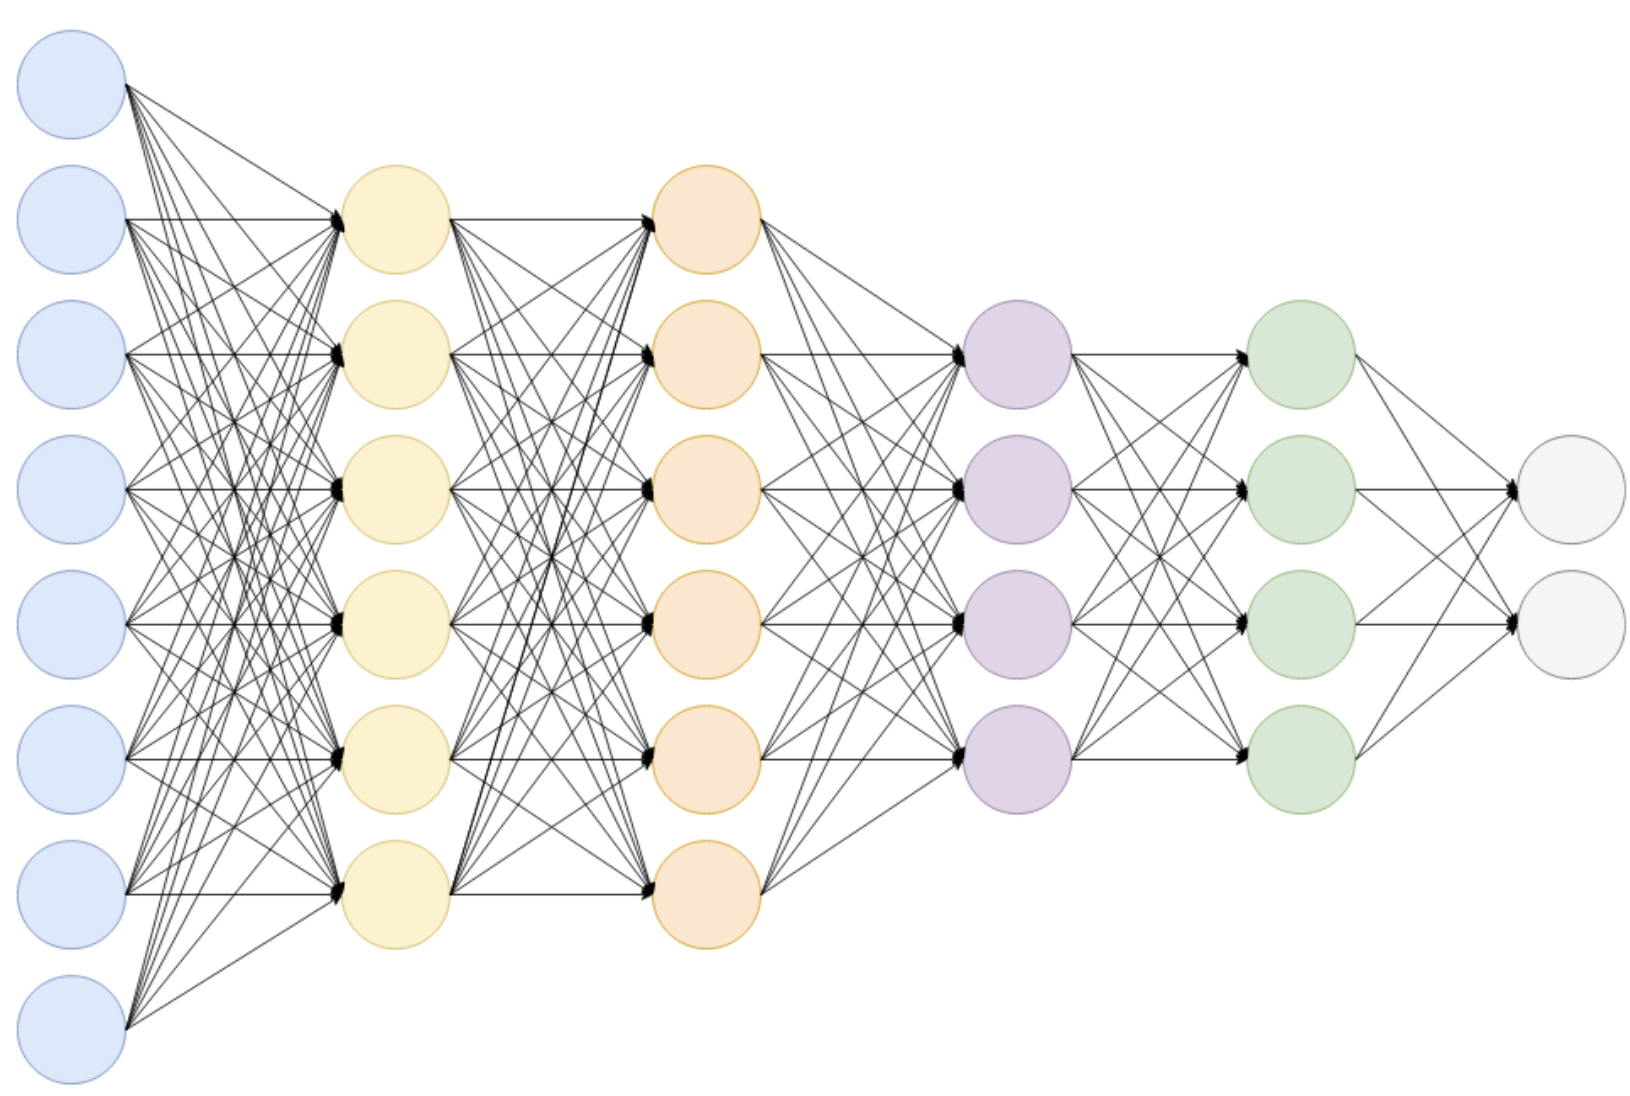
\includegraphics[width=0.8\textwidth]{Images/DataMining/CNNandFCLayers}
	\caption{CNN and FC layers \cite{Win:2023}} \label{fig:CNNandFCLayers}
\end{figure}


A critical stage in the feature extraction process is convolution. Convolution produces maps of features. By adding zero values to the input, padding makes the border less likely to cause information loss. To regulate the convolution density, stride is used. Feature maps created after convolution may cause overfitting, which calls for pooling (either maximum or average pooling) to get rid of redundant data. Figure \ref{fig:ProcedureCNN} shows the overall CNN technique. Here is an explanation of what padding, stride, and pooling mean \cite{Li:2021}:

\begin{itemize}
	\item \textbf{Padding:} Padding involves adding extra border pixels to the input image before convolution. This is done by appending additional rows and columns of zero values around the image. The purpose of padding is to mitigate information loss at the borders during convolutional operations.
	
	\item \textbf{Stride:} Stride is the step size or the number of pixels by which the convolutional filter moves across the input image during the convolution operation. A larger stride reduces the spatial dimensions of the feature maps, leading to a more compact representation.
	
	\item \textbf{Pooling:} Pooling is a down-sampling operation applied after convolution. It reduces the spatial dimensions of the feature maps, helping to control the number of parameters in the network. Pooling is typically performed using operations such as max pooling or average pooling \cite{Win:2023}.
	
	\begin{enumerate}
		\item \textbf{Max Pooling:} Max pooling is a specific pooling operation where, for each region of the feature map, the maximum value is taken. This helps retain the most significant information from that region, providing a form of spatial summarization.
		
		\item \textbf{Average Pooling:} Average pooling is another type of pooling operation where, for each region of the feature map, the average value is computed. This operation helps reduce the spatial dimensions while maintaining a smoother and less detailed representation.
	\end{enumerate}
\end{itemize}


\begin{figure}[h!]
	\centering
	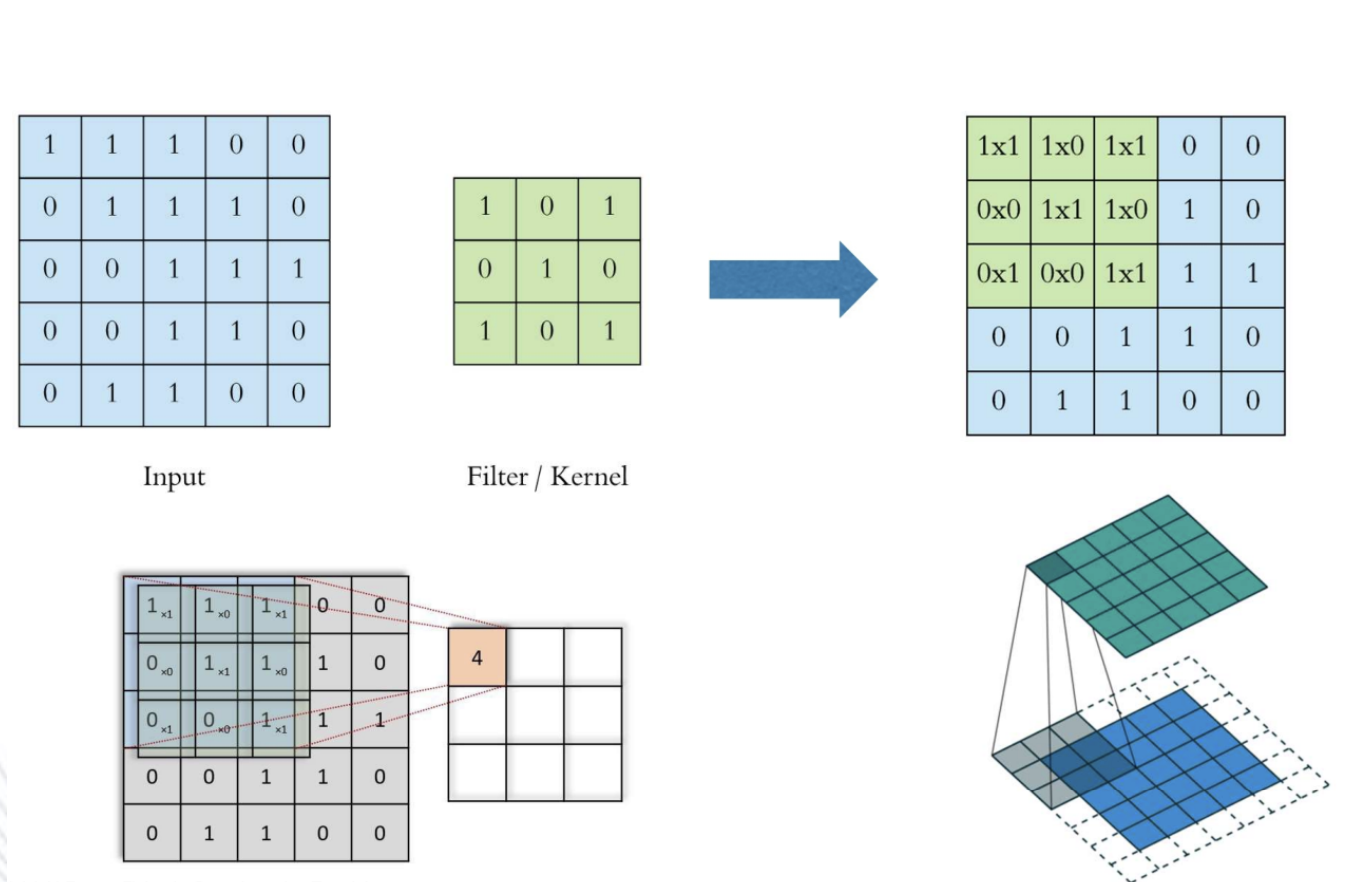
\includegraphics[width=0.8\textwidth]{Images/DataMining/ProcedureCNN}
	\caption{Procedure of a two-dimensional CNN \cite{Win:2023}} \label{fig:ProcedureCNN}
\end{figure}

There are many different architectural variants in the field of Convolutional Neural Networks (CNNs), but their essential elements are always very similar. Using the well-known LeNet-5 as an example, it consists of three essential layers: fully-connected, pooling, and convolutional layers \cite{Gu:2018}. The convolutional layer's main objective is to extract feature representations from the inputs.

The convolutional layer, as shown in Figure \ref{subfig:LetNet5ArchitectureNetwork}, is made up of numerous convolution kernels that are responsible for creating unique feature maps. Each neuron in a feature map connects to a neighbourhood of neurons in the preceding layer, which is known as the neuron's receptive field. The process of creating a feature map begins with convolving the input with a learnt kernel, followed by applying an element-wise nonlinear activation function to the results. It is vital to note that each feature map is formed by sharing the kernel across all spatial regions of the input, resulting in the use of numerous distinct kernels for the entire set of feature maps.

\begin{figure}[h!]
	\centering
	
	\begin{subfigure}{0.65\textwidth}
		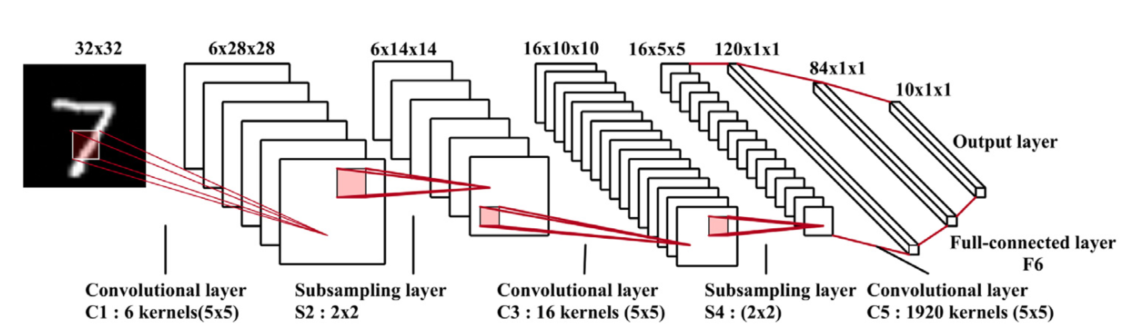
\includegraphics[width=\linewidth]{Images/DataMining/LetNet5ArchitectureNetwork}
		\caption{LetNet-5 network}    % \caption{} is kept to keep (a), (b), (c) etc. below each subfigure.
		\label{subfig:LetNet5ArchitectureNetwork}
	\end{subfigure}
	\hfill
	\begin{subfigure}{0.3\textwidth}
		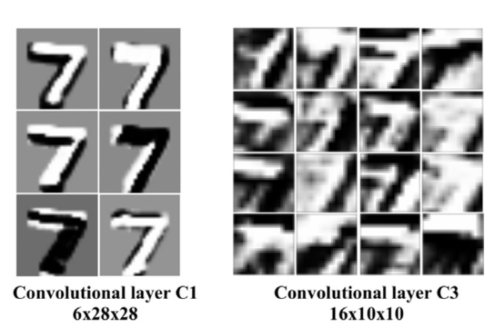
\includegraphics[width=\linewidth]{Images/DataMining/LetNet5ArchitectureLearnedFeatures}
		\caption{Learned features}    % \caption{} is kept to keep (a), (b), (c) etc. below each subfigure.
		\label{subfig:LetNet5ArchitectureLearnedFeatures}
	\end{subfigure}
	
	\caption{The architecture of the LeNet-5 network \cite{Gu:2018}. (\subref{subfig:LetNet5ArchitectureNetwork}) The architecture of the LeNet-5 network, renowned for its effectiveness in digit classification tasks. (\subref{subfig:LetNet5ArchitectureLearnedFeatures}) Displaying the features within the LeNet-5 network through visualizations, where each layer's feature maps are showcased in distinct blocks.}
	\label{fig:LetNet5Architecture}
\end{figure}

Mathematically, the feature value at location $(i, j)$ in the $k$th feature map of the $l$th layer (denoted as $z^l_{i,j,k}$) is computed by the expression:

\begin{equation}
	z^l_{i,j,k} = {\mathbf{w}^l_k}^T \mathbf{x}^l_{i,j} + b^l_k
\end{equation}

Where $\mathbf{w}^l_k$ and $ b^l_k$ represent the weight vector and bias term of the $k$th filter of the $l$th layer, while $\mathbf{x}^l_{i,j}$ is the input patch centered at location $(i, j)$ of the $l$th layer. The weight sharing mechanism, where the kernel generating the feature map is shared, offers advantages such as reducing model complexity and facilitating network training.

The activation function ($a(\cdot)$) introduces nonlinearity to the CNN, which is crucial for detecting nonlinear features in multi-layer networks. The activation value ($a_{l,i,j,k}$) of the convolutional feature $z_{l,i,j,k}$ is computed as:

\begin{equation}
	a^l_{i,j,k} = a(z^l_{i,j,k})
\end{equation}

Common activation functions include sigmoid, tanh, and ReLU. More information about activation functions is given in Subsection \ref{subsection:ActivationFunction}. The pooling layer, positioned between convolutional layers, aims to achieve shift-invariance by downsampling the feature maps' resolution. Each feature map in the pooling layer connects to its corresponding feature map in the preceding convolutional layer. The pooling operation, denoted as $\mathrm{pool}(\cdot)$, is applied to each feature map $a^l_{m,n,k}$ with:

\begin{equation}
	y^l_{i,j,k} = \mathrm{pool}(a^l_{m,n,k}), \forall (m, n) \in \mathcal{R}_{ij}
\end{equation}

Here, $\mathcal{R}_{ij}$ represents a local neighborhood around location $(i, j)$. Common pooling operations include average pooling and max pooling. The learned feature maps, as demonstrated in Figure \ref{subfig:LetNet5ArchitectureLearnedFeatures} for the digit 7, progressively capture hierarchical features, with early layers detecting low-level features like edges and curves, and subsequent layers encoding more abstract features.

Following the convolutional and pooling layers, one or more fully-connected layers may be present to perform high-level reasoning. These layers connect all neurons from the previous layer to every neuron in the current layer, generating global semantic information. Notably, a fully-connected layer can be replaced by a $1 \times 1$ convolution layer.

The final layer in CNNs is the output layer. For classification tasks, the softmax operator (see Subsection \ref{subsection:outputCNN}) is commonly employed (See \ref{subsec}). Alternatively, SVM can be combined with CNN features to address diverse classification tasks. Consider a set of $N$ desired input-output relationships represented as $\{(\mathbf{x}^{(n)}, \mathbf{y}^{(n)}); n \in [1, \ldots, N]\}$. The parameters of a CNN, denoted as $\mathbf{\theta}$, including weight vectors and bias terms, are optimized by minimizing an appropriate loss function defined for the specific task:

\begin{equation}
	\mathcal{L} = \frac{1}{N} \sum_{n=1}^{N} \ell(\mathbf{\theta}; \mathbf{y}^{(n)}, \mathbf{o}^{(n)})
\end{equation}

Here, $\mathcal{L}$ represents the loss function, which quantifies the discrepancy between the predicted output ($\mathbf{o}^{(n)}$) and the actual target label ($\mathbf{y}^{(n)}$) for $n$th input data point $\mathbf{x}^{(n)}$. The symbol $\mathbf{\theta}$ denotes all the parameters of the CNN, including weight vectors and bias terms. The function $\ell(\mathbf{\theta}; \mathbf{y}^{(n)}, \mathbf{o}^{(n)})$ is the individual loss for a specific data point, measuring the dissimilarity between the predicted output and the true label. The goal during training is to minimize the average loss over all data points, achieved through techniques such as stochastic gradient descent. Additional details about loss functions are available in Subsection \ref{subsection:LossFunction}.

The training of a CNN involves global optimization, with the aim of finding the best set of parameters by minimizing the loss function. Stochastic gradient descent emerges as a common solution for optimizing CNN networks, providing an effective means of iterative parameter adjustment. Optimizing is explained in the Subsection \ref{subsection:optimizer}. 

\subsection{Activation Function}
\label{subsection:ActivationFunction}

Convolutional Neural Networks (CNNs) leverage various activation functions to express intricate features \cite{Li:2021}. Functioning akin to the human brain's neuron model, the activation function serves as a unit determining the transmission of information to the next neuron. In a multilayer neural network, an activation function exists between two layers, structurally depicted in Figure \ref{fig:activationFunctionStructure}.

In Figure \ref{fig:activationFunctionStructure}, $x_i$ denotes input features, $n$ features simultaneously input to neuron $j$, $w_{ij}$ represents connection weight between input feature $x_i$ and neuron $j$, $b_j$ is the internal state (bias) of neuron $j$, and $y_j$ is the neuron's output. The activation function, denoted as $f(·)$ , includes options like the sigmoid, tanh, rectified linear unit (ReLU), and others.

When no activation function or a linear function is used, the network output is a linear combination of inputs, limiting learning ability. Nonlinear activation functions, like sigmoid and tanh, are introduced to enhance the network's capability to fit data.

\begin{figure}[h!]
	\centering
	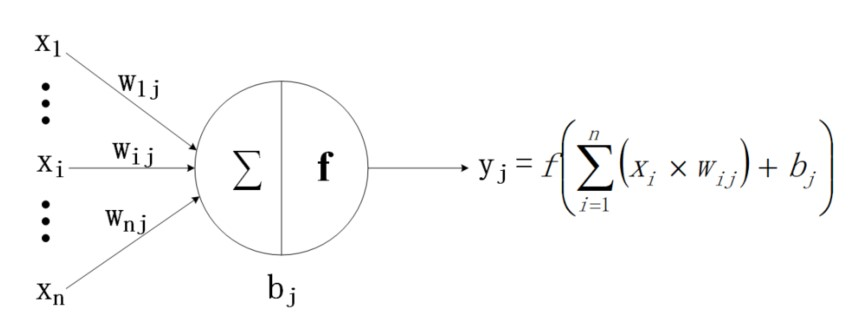
\includegraphics[width=0.6\textwidth]{Images/DataMining/activationFunctionStructure}
	\caption{Overall structure of an activation function \cite{Li:2021}.} \label{fig:activationFunctionStructure}
\end{figure}

Some of the well-known actiovatoion functions are shown in the Figure \ref{fig:activationFunctions}. The sigmoid function maps a real number to (0, 1), suitable for binary classification. The tanh function maps to (-1, 1), aiding normalization. ReLU, with its advantages in learning speed, is preferred in deep networks. Leaky ReLU and PReLU address limitations of ReLU, reducing neuron inactivation. ELU improves convergence by having a negative output average.

Swish, proposed by Google, and mish, a novel activation function, demonstrate improved performance compared to ReLU and Swish in deeper models across diverse datasets. mish, in particular, exhibits superior gradient flow, accuracy, and generalization properties. Experimental results consistently support the effectiveness of Mish across standard architectures.

\begin{figure}[h!]
	\centering
	
	\begin{subfigure}{0.22\textwidth}
		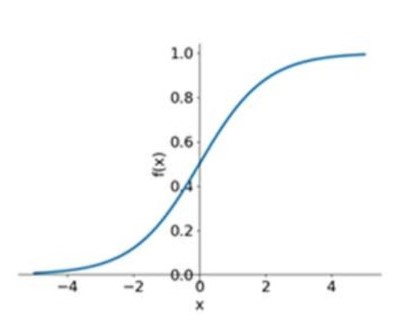
\includegraphics[width=\linewidth]{Images/DataMining/SigmoidFunction}
		\caption{}    % \caption{} is kept to keep (a), (b), (c) etc. below each subfigure.
		\label{subfig:Sigmoid}
	\end{subfigure}
	\hfill
	\begin{subfigure}{0.22\textwidth}
		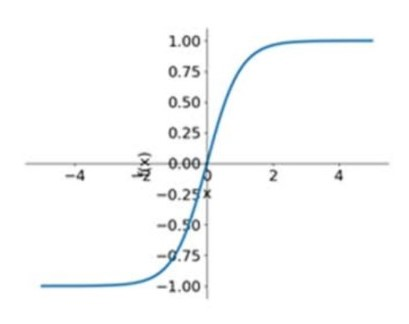
\includegraphics[width=\linewidth]{Images/DataMining/TanhFunction}
		\caption{}    % \caption{} is kept to keep (a), (b), (c) etc. below each subfigure.
		\label{subfig:Tanh}
	\end{subfigure}
	\hfill
	\begin{subfigure}{0.22\textwidth}
		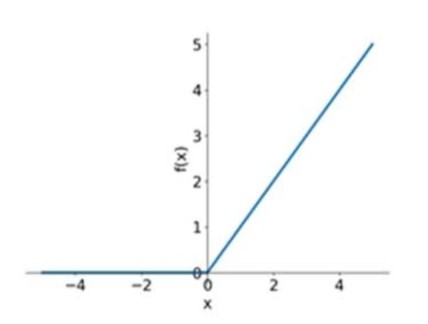
\includegraphics[width=\linewidth]{Images/DataMining/ReLUFunction}
		\caption{}    % \caption{} is kept to keep (a), (b), (c) etc. below each subfigure.
		\label{subfig:ReLU}
	\end{subfigure}
	\hfill
	\begin{subfigure}{0.22\textwidth}
		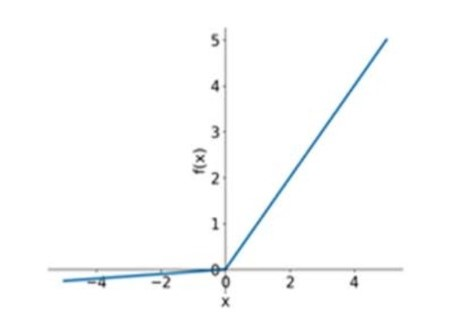
\includegraphics[width=\linewidth]{Images/DataMining/LeakyReLUFunction}
		\caption{}    % \caption{} is kept to keep (a), (b), (c) etc. below each subfigure.
		\label{subfig:LeakyReLU}
	\end{subfigure}
	
	\medskip
	
	\begin{subfigure}{0.22\textwidth}
		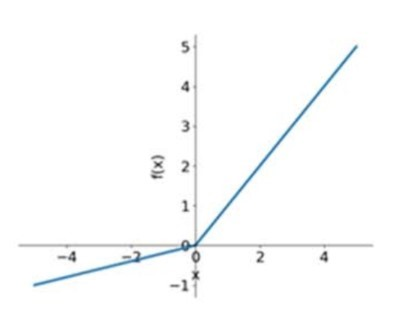
\includegraphics[width=\linewidth]{Images/DataMining/PReLUFunction}
		\caption{}    % \caption{} is kept to keep (a), (b), (c) etc. below each subfigure.
		\label{subfig:PReLU}
	\end{subfigure}
	\hfill
	\begin{subfigure}{0.22\textwidth}
		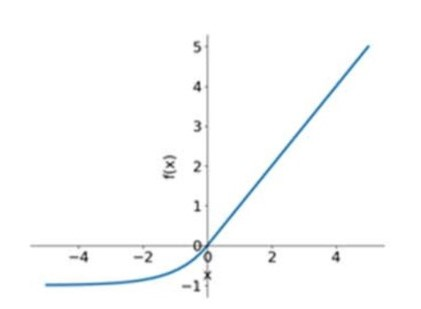
\includegraphics[width=\linewidth]{Images/DataMining/ELUFunction}
		\caption{}    % \caption{} is kept to keep (a), (b), (c) etc. below each subfigure.
		\label{subfig:ELU}
	\end{subfigure}
	\hfill
	\begin{subfigure}{0.22\textwidth}
		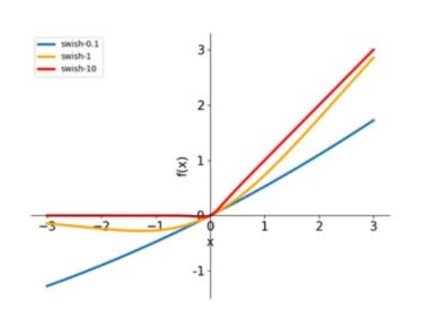
\includegraphics[width=\linewidth]{Images/DataMining/SwishFunctions}
		\caption{}    % \caption{} is kept to keep (a), (b), (c) etc. below each subfigure.
		\label{subfig:Swish}
	\end{subfigure}
	\hfill
	\begin{subfigure}{0.22\textwidth}
		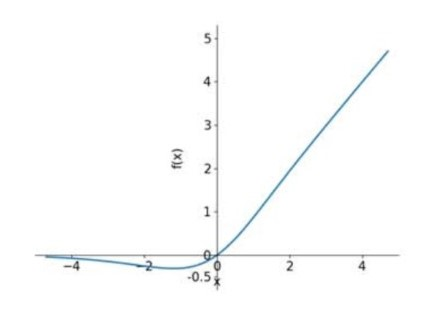
\includegraphics[width=\linewidth]{Images/DataMining/MishFunction}
		\caption{}    % \caption{} is kept to keep (a), (b), (c) etc. below each subfigure.
		\label{subfig:Mish}
	\end{subfigure}
	
	\caption{Diagrams of activation functions \cite{Li:2021}.  (\subref{subfig:Sigmoid}) Sigmoid function.  (\subref{subfig:Tanh}) Tanh function. (\subref{subfig:ReLU}) ReLU function. (\subref{subfig:LeakyReLU}) Leaky ReLU function. (\subref{subfig:PReLU}) PReLU function. (\subref{subfig:ELU}) ELU function.  (\subref{subfig:Swish}) Swish function. (\subref{subfig:Mish}) Mish function.}
	\label{fig:activationFunctions}
\end{figure}

\subsubsection{Guidelines for Activation Function Selection}

\begin{enumerate}
	\item For binary classification tasks, employ the sigmoid function in the last layer; for multiclassification, opt for the softmax function.
	\item Exercise caution with sigmoid and tanh functions due to potential gradient vanishing issues. Preferably, in hidden layers, consider ReLU or leaky ReLU for improved performance.
	\item When uncertain about the suitable activation function, consider experimenting with ReLU or leaky ReLU as reliable starting points.
	\item In cases where numerous neurons become inactive during training, explore alternatives like leaky ReLU, PReLU, or similar activation functions to address the issue.
	\item To expedite training, set the negative slope in leaky ReLU to 0.02, mitigating potential challenges associated with a slow convergence rate.
\end{enumerate}


\subsection{Loss Function}
\label{subsection:LossFunction}

The loss function, crucial in calculating the disparity between predicted and actual values, serves as a learning criterion for optimization in CNNs. It plays a key role in regression and classification problems, aiming to minimize the loss. Commonly used loss functions include Mean Absolute Error (MAE), Mean Square Error (MSE), and Cross Entropy \cite{Li:2021}.

	\begin{itemize}
		
		\item \textbf{Loss Function for Regression}
	
		In CNNs, MAE or MSE is commonly used for regression problems. MAE computes the mean absolute error, providing robustness to outliers. On the other hand, MSE calculates the mean of square errors, enabling controlled update rates. Choosing between them depends on the presence of outliers in the training set.
		
		\item \textbf{Loss Function for Classification}
		
		Various loss functions are employed in CNNs for classification tasks. The widely used cross entropy loss evaluates the difference between predicted probability distributions and actual distributions. While effective, it has limitations, focusing solely on classification correctness and neglecting factors like compactness within classes and margins between different classes.
		
		\begin{itemize}
			\item \textbf{Contrastive Loss:}
			Enlarges distance between different categories and minimizes distance within the same categories, often used in dimensionality reduction for face recognition.
			
			\item \textbf{Triplet Loss:}
			Introduced for better face embeddings, minimizes the distance between anchor and positive images while increasing the distance to negative ones. Useful in fine-grained classification at the individual level.
			
			\item \textbf{Center Loss:}
			An improvement upon cross entropy, focuses on the uniformity of distribution within the same class by minimizing intraclass differences.
		\end{itemize}
		
		These diverse loss functions offer flexibility and cater to specific challenges encountered in regression and classification tasks within CNNs.
		
		\item \textbf{Guidelines for Loss Function Selection}
		\label{Loss Function}
		\begin{enumerate}
			\item For regression challenges in CNN models, viable choices for the loss function include L1 loss or L2 loss.
			
			\item When confronted with classification tasks, opt for a suitable loss function from the available options.
			
			\item Cross entropy loss stands out as a prevalent choice, frequently employed in CNN models featuring a softmax layer at the conclusion.
			
			\item Addressing concerns regarding compactness within a class or the margin between different classes necessitates considering enhancements based on cross entropy loss. Examples include center loss and large-margin softmax loss.
			
			\item The choice of a loss function in CNNs should align with the specific application scenario. For instance, in face recognition applications, contrastive loss and triplet loss have emerged as commonly utilized options.
		\end{enumerate}
	
	\end{itemize}

\subsection{Optimizer}
\label{subsection:optimizer}

In CNNs, optimization of nonconvex functions is crucial, often necessitating optimizers to efficiently minimize the loss function within a reasonable timeframe \cite{Li:2021}. Nonconvex functions exhibit intricate landscapes with multiple local optima, making their optimization challenging. These functions lack the convex property, where any line segment connecting two points lies entirely within the function's domain, complicating the search for the global minimum.

\subsubsection{Gradient Descent}

Three gradient descent methods for training CNN models are batch gradient descent (BGD), stochastic gradient descent (SGD), and mini-batch gradient descent (MBGD).

\begin{itemize}
	\item BGD is slow due to calculating the average gradient of the entire batch, making it impractical for large datasets or in-memory constraints.
	\item SGD, using one sample per update, is suitable for online learning but prone to high variance and oscillations.
	\item MBGD, a popular choice, combines advantages of BGD and SGD, efficiently using a small batch to stabilize convergence.
\end{itemize}

	\begin{itemize}
		\item \textbf{Gradient Descent Optimization Algorithms}
		
		Effective algorithms built on MBGD include:
		
		\begin{itemize}
			\item Momentum algorithm simulates physical momentum, preventing oscillations for faster convergence.
			\item Nesterov accelerated gradient (NAG) enhances momentum algorithm predictability to slow down before positive slopes.
			\item Adagrad adapts the learning rate to parameters, suitable for sparse data.
			\item Adadelta limits the monotonically decreasing learning rate of Adagrad.
			\item RMSprop addresses diminishing learning rate issues in Adagrad.
			\item Adam combines momentum with RMSprop, proving effective in various CNN structures.
			\item Other variants like AdaMax, Nadam, and AMSGrad offer improvements and constraints.
		\end{itemize}
		
	\item \textbf{Guidelines for Optimizer Selection:}
		
		\begin{enumerate}
			\item Utilize Mini-Batch Gradient Descent (MBGD) to strike a balance between Batch Gradient Descent (BGD) and Stochastic Gradient Descent (SGD), considering both computing cost and the accuracy of each update.
			
			\item Optimizer performance is intricately linked to data distribution. Adhering to the No Free Lunch Theorem, no single optimizer universally outperforms others in all scenarios. A prudent approach involves selecting optimizers based on their unique characteristics.
			
			\item In instances of excessive oscillation or divergence, it is advisable to contemplate reducing the learning rate to address these issues.
		\end{enumerate}
		
	\end{itemize}


\section{Applications}

The utilization of Convolutional Neural Networks (CNN) in computer vision has made possible achievements that were once deemed impossible over the past centuries. These accomplishments include facial recognition, autonomous vehicles, self-service supermarkets, and intelligent medical treatments \cite{Li:2021}.

\subsection{1-D CNN Applications}

\begin{enumerate}
	\item \textbf{Time Series Prediction:}
	\begin{itemize}
		\item Applied to predict time series data, such as electrocardiogram (ECG) time series, weather forecast, and traffic flow prediction.
		\item Example: Prediction of atrial fibrillation using short-term ECG data.
	\end{itemize}
	
	\item \textbf{Signal Identification:}
	\begin{itemize}
		\item Used for discriminating input signals based on features learned from training data.
		\item Applications include ECG signal identification, structural damage identification, and system fault identification.
	\end{itemize}
\end{enumerate}

\subsection{2-D CNN Applications}

\textbf{Magic Wand Project:} The application of artificial neural networks extends its influence into diverse consumer-centric projects, notably exemplified in the domain of interactive devices, such as the magic wand project. Within this context, the magic wand serves as an intuitive input device, enabling users to command and control various functionalities through gestures. While gesture recognition technology has historical roots, the integration of artificial neural networks into such applications gained prominence around the 2010s, revolutionizing the accuracy and responsiveness of gesture-based interfaces. Unlike traditional approaches relying on rule-based systems, the introduction of neural networks enhanced the magic wand's capability to recognize and interpret intricate hand movements, thus significantly advancing user interaction and experience. A crucial aspect of the magic wand project involves real-time processing of sensor data, demanding efficient neural network architectures capable of swiftly interpreting gesture patterns and translating them into actionable commands. Consequently, the incorporation of artificial neural networks has been instrumental in elevating the magic wand project to new heights of interactivity and usability \cite{Set:2023}. 

Moreover, the consideration of user privacy remains paramount, necessitating the implementation of safeguards to ensure that data processing occurs only when specific predefined gestures, acting as keywords, are identified by the neural network. This strategic approach not only enhances the device's efficiency by reducing unnecessary data transmission but also addresses critical privacy concerns associated with continuous sensor monitoring, thereby establishing a robust and responsible foundation for the magic wand project \cite{Set:2023}.

\textbf{Other 2-D applications of CNNs are:}

\begin{enumerate}
	\item Image Classification

	\item Object Detection
	
	\item Image Segmentation
	
	\item Face Recognition

\end{enumerate}

\subsection{Multidimensional CNN Applications}

\begin{enumerate}
	\item \textbf{Human Action Recognition:}  \cite{Mard:2017}
	\begin{itemize}
		\item Involves recognizing human actions in videos.
		\item 3D CNNs used to extract features, and integration with 2D CNN features is discussed.
	\end{itemize}
	
	\item \textbf{Object Recognition/Detection in 3D:}
	\begin{itemize}
		\item Applications like object detection of RGBD images using 3D ShapeNet and VoxNet for 3D object recognition.
		\item Detection of high-dimensional images like X-rays and CT images using 3D CNN.
	\end{itemize}
\end{enumerate}


\section{Why CNN?}

Selecting a Convolutional Neural Network (CNN) architecture for the magic wand project is a well-justified decision based on the unique characteristics of the input data sensor readings or gesture patterns (refer to Section \ref{subsection:InputDataMagicWand}). In the magic wand project, the input data is often represented as multidimensional arrays, reflecting the readings from various sensors capturing the gesture dynamics. CNNs, specifically designed for handling multidimensional tensors, are particularly adept at extracting relevant features from relationships within such data structures \cite{War:2020}.

CNNs, commonly recognized for their success in image processing tasks, exhibit a remarkable ability to learn hierarchical features. Importantly, the versatility of CNNs extends beyond traditional image data, making them highly suitable for processing any form of multidimensional vector input.

Considering that the data generated by the magic wand project shares similarities with images being represented as two-dimensional grids CNNs emerge as a natural and effective choice. The network's inherent capability to capture relationships within a two-dimensional space aligns seamlessly with the structure of the sensor readings or gesture patterns. Consequently, employing CNNs in the magic wand project facilitates the extraction of meaningful features from the input data, enabling the neural network to discern and interpret intricate gesture patterns with precision and efficacy \cite{Xu:2022}.

\section{Hyperparameters}

Tuning activation functions, loss functions, and optimizers, as well as altering many other hyperparameters, all have a significant impact on model performance. It is well understood that no universally determined collection of hyperparameters ensures optimal solutions at all times. As a result, when navigating the difficult process of hyperparameter tuning, relying on a combination of experience and set rules becomes critical \cite{Li:2021}.

\begin{itemize}

	\item \textbf{Learning Rate:} The learning rate in the context of the magic wand project pertains to the step size at which the neural network updates its weights during training. It should be carefully chosen within an appropriate range to balance convergence speed and stability, optimizing the model's ability to recognize and interpret intricate gesture patterns.
	
	\item \textbf{Epoch:} In the magic wand project, the epoch signifies the number of times the entire dataset of gesture samples is fed into the neural network for training. The choice of epochs should be adjusted based on the observed gap between training set and validation set accuracy. This ensures the prevention of underfitting or overfitting and fine-tunes the network for accurate gesture recognition.
	
	\item \textbf{Mini-Batch Size:} Referring to the number of gesture samples sent to the model in each training iteration, the mini-batch size plays a crucial role in convergence and stability. For optimal performance on the Arduino Nano, it is advisable to set a batch size that aligns with the device's computational capacity, balancing efficiency and accuracy in recognizing gestures.
	
	\item \textbf{Number of Conv Layers:} In the context of the magic wand project, the number of convolutional layers determines the depth of the network and its capacity to capture various levels of features present in gesture patterns. Careful consideration is needed to find the right balance, as increasing layers generally allows the representation of more complex features but may pose challenges during training.
	
	\item \textbf{Conv Kernel Size:} The size of convolution kernels in each layer is a crucial hyperparameter affecting the network's capacity and computational complexity. Commonly used kernel sizes, such as 3x3 or 1x1, should be chosen to suit the intricacies of gesture data, ensuring effective feature extraction and representation.
	
	\item \textbf{Number of Filters (Kernels):} The number of filters in each convolutional layer determines the depth and capacity of the neural network for recognizing gesture patterns. This hyperparameter often increases in deeper layers to capture and understand more nuanced features in the magic wand's input data.
	
	\item \textbf{Activation Function:} The activation function introduces non-linearity to the network, a crucial aspect for capturing complex relationships in gesture data. For the magic wand project, the choice of activation function, such as ReLU or Sigmoid, should align with the nature of the gesture recognition problem and characteristics of the input data.
	
\end{itemize}


\section{Requirements}
	\begin{itemize}
		\item \textbf{Input Format:} 
		Configure the CNN to adeptly handle the specific format and characteristics of sensor data generated by the magic wand, optimizing for the limited input data capabilities of the Arduino Nano.
		
		\item \textbf{Real-time Processing:} 
		Optimize the CNN architecture for real-time processing, ensuring timely recognition and response to gesture patterns in dynamic scenarios encountered by the Arduino Nano \cite{Munoz:2019}.
		
		\item \textbf{Energy Efficiency:} 
		Design an energy-efficient CNN model that minimizes power consumption during gesture recognition without compromising performance, acknowledging the limited power resources available on the Arduino Nano.
		
		\item \textbf{Output Interface:}
		Align the CNN's output format with the capabilities of the magic wand and Arduino Nano, facilitating seamless integration and utilization of the device's limited output capabilities for effective gesture-based interactions.
		
		\item \textbf{Noise Robustness:} 
		Implement features or preprocessing steps in the CNN to enhance noise robustness, adapting to different environments and addressing potential variability in sensor readings associated with varying conditions \cite{Munoz:2019}.
		
		\item \textbf{Inference Speed:}
		Optimize the CNN for fast inference to ensure prompt recognition of gestures, considering the limited processing speed of the Arduino Nano and the need for swift response times.
		
		\item \textbf{Training Considerations:} 
		Design the CNN to be trainable with a manageable amount of gesture data, considering the limited availability of training data for the magic wand and addressing the specific nuances of the intended gesture recognition application.
		
		\item \textbf{Postprocessing Techniques:} 
		Implement postprocessing methods, such as consensus-based recognition or temporal filtering, to refine and enhance the accuracy of gesture recognition in real-world scenarios, accommodating uncertainties and variations.
		
		\item \textbf{Compatibility:} 
		Ensure that the CNN model architecture and parameters are compatible with the hardware specifications of the Arduino Nano, allowing for seamless integration and optimal performance in the context of the magic wand project.

	\end{itemize}


\section{Input}

Understanding the complexities of input data is critical for effective model construction and training in the world of Convolutional Neural Networks (CNNs). The structure of the input data is depicted below, emphasising its significance as a multi-dimensional array also known as a tensor \cite{Xu:2022}.


\subsection{Input Data Specifications}


\subsubsection{Dimensions for Image Data}

The input data in a Convolutional Neural Network (CNN) is fundamentally structured as a multi-dimensional array, commonly referred to as a tensor. This tensor represents the raw input to the neural network and is pivotal for subsequent feature extraction and hierarchical representation learning \cite{War:2020}.

\subsubsection{Input Shape Specifications}

For image data, the tensor dimensions typically encompass the height, width, and channels of the image. In the context of color images using the RGB color space, the shape of the tensor is commonly denoted as (height, width, 3). Here, "height" and "width" correspond to the spatial dimensions of the image, and "3" indicates the three color channels (Red, Green, Blue). For example, if you have an image with dimensions $100 \times 100$ pixels, the RGB representation would be a $100 \times 100 \times 3$ matrix, where each element corresponds to the intensity of the respective color channel at that pixel.

in the code presented in the Section \ref{section:DataMiningExampleCode}, in Listing ??. In this example, \texttt{height}, \texttt{width}, and \texttt{channels} are replaced with the actual dimensions of the input images. More is explained in the Section \ref{section:DataMiningExampleCode}.


Grayscale images, on the other hand, have only one channel. Each pixel in a grayscale image is represented by a single value indicating the intensity of brightness. The range of intensity values depends on the bit depth; for an 8-bit image, values typically range from 0 (black) to 255 (white). The matrix representing a grayscale image would be a 2D matrix, where each element represents the intensity of a pixel. In the Figure \ref{fig:DigitalImage} the digital presentation of the number "4" is presented. Note that the pixel values are normalized to be between 0 and 1, with 0 representing the black color and 1 representing the white color pixel value. 


\begin{figure}[h!]
	\centering
	
	\begin{subfigure}{0.45\textwidth}
		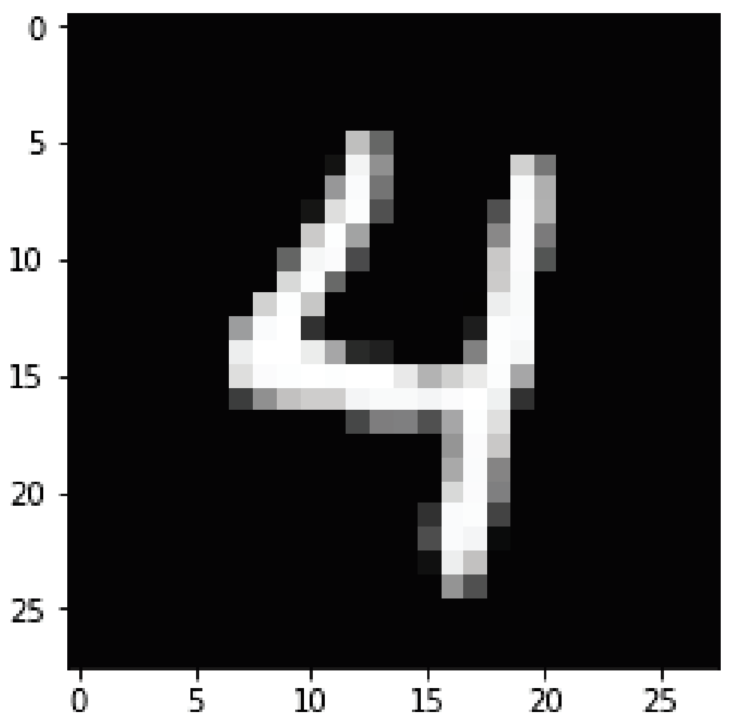
\includegraphics[width=\linewidth]{Images/DataMining/DigitalImage}
		\caption{}    % \caption{} is kept to keep (a), (b), (c) etc. below each subfigure.
		\label{subfig:DigitalImage}
	\end{subfigure}
	\hfill
	\begin{subfigure}{0.45\textwidth}
		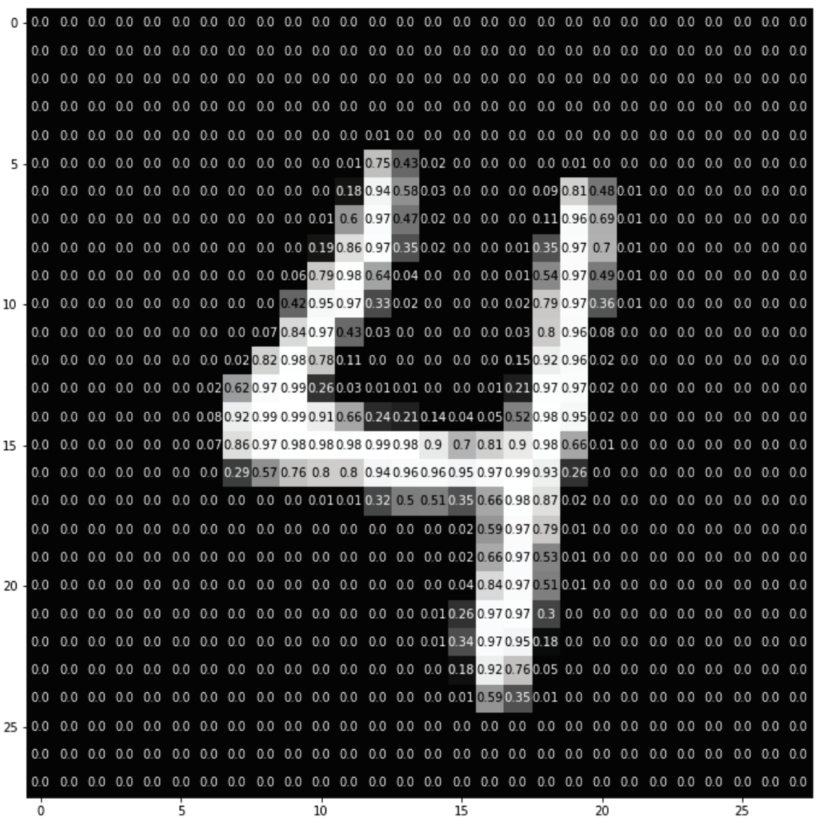
\includegraphics[width=\linewidth]{Images/DataMining/DigitalImagePixelValues}
		\caption{}    % \caption{} is kept to keep (a), (b), (c) etc. below each subfigure.
		\label{subfig:DigitalImagePixelValues}
	\end{subfigure}
	
	\caption{Digital presentation of an image \cite{Sewak:2018}. (\subref{subfig:DigitalImage}) Digital presentation of the number "4." (\subref{subfig:DigitalImagePixelValues}) Normalized pixel values of the number "4."}
	\label{fig:DigitalImage}
\end{figure}

% change
\subsection{Input Data for Magic Wand}
\label{subsection:InputDataMagicWand}

In our time-series accelerometer data, adjacent accelerometer readings give us clues about the device’s motion. For example, if acceleration on one axis changes rapidly from zero to positive, then back to zero, the device might have begun motion in that direction. \ref{Fig:5.7} shows a hypothetical example of this.

\begin{figure}[h!]
	
	\centering
	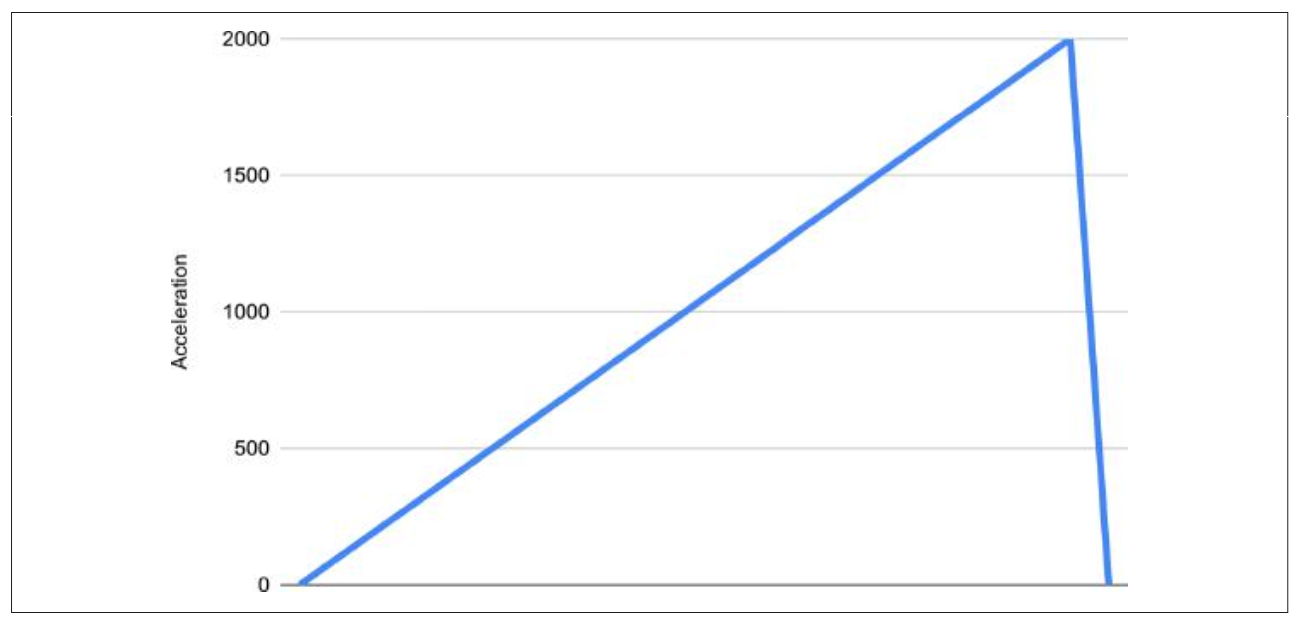
\includegraphics[width=\textwidth]{Images/DataMining/Accelerometervalues1}
	\caption{\textbf{Accelerometer values for a single axis of a device being moved} \cite{War:2020}}
	\label{Fig:5.7}
\end{figure}

Any given gesture is composed of a series of motions, one after the other. For exam‐ ple, consider our “wing” gesture, shown in \ref{Fig:5.9}

The device is first moved down and to the right, then up and to the right, then down and to the right, then up and to the right again. \ref{Fig:5.8} shows a sample of real data captured during the “wing” gesture, measured in milli-Gs.

\begin{figure}[h!]
	
	\centering
	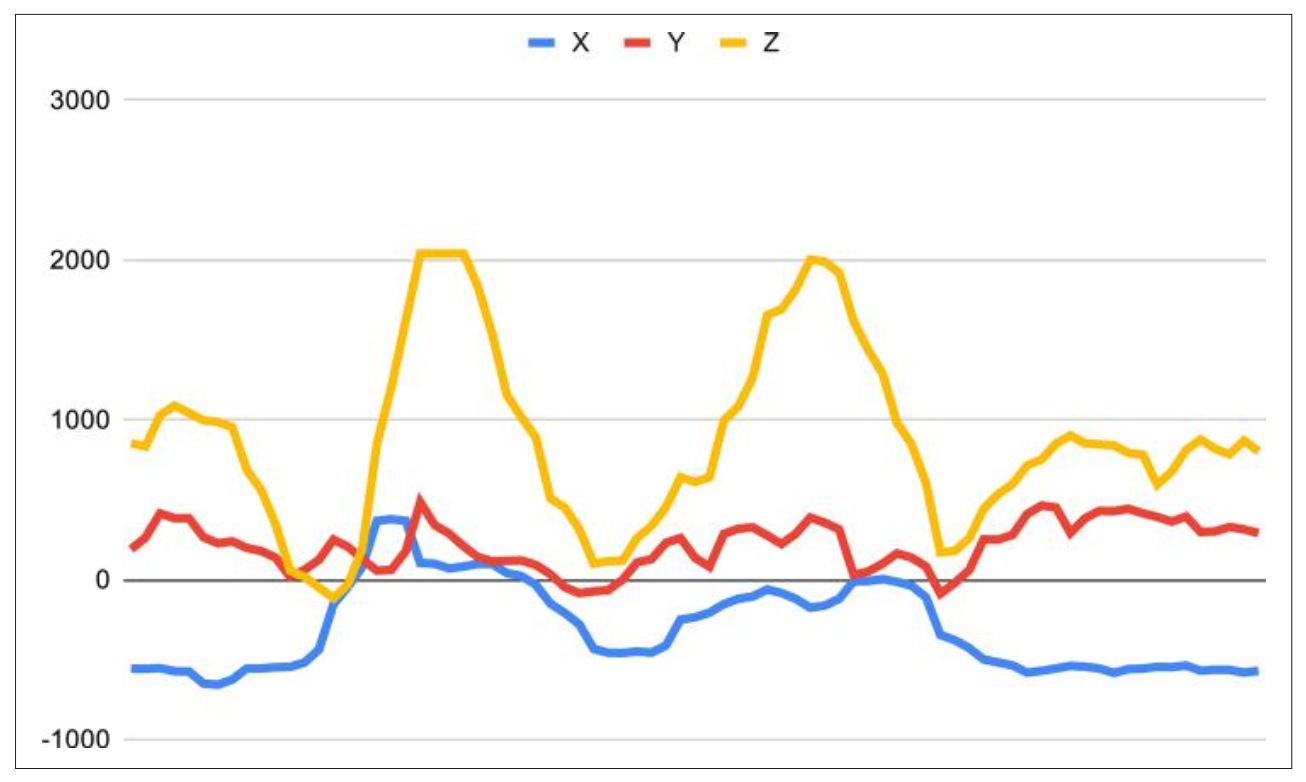
\includegraphics[width=\textwidth]{Images/DataMining/Accelerometervalues2}
	\caption{\textbf{Accelerometer values during the “wing” gesture} \cite{War:2020}}
	\label{Fig:5.8}
\end{figure}

By looking at this graph and breaking it down into its component parts, we can understand which gesture is being made. From the z-axis acceleration, it’s very clear that the device is being moved up and down in the way we would expect given the “wing” gesture’s shape. More subtly, we can see how the acceleration on the x-axis correlates with the z-axis changes in a way that indicates the device’s motion across the width of the gesture. Meanwhile, we can observe that the y-axis remains mostly stable.

Similarly, a CNN with multiple layers is able to learn how to discern each gesture through its telltale component parts. For example, a network might learn to distin‐ guish an up-and-down motion, and that two of them, when combined with the appropriate z- and y-axis movements, indicates a “wing” gesture \cite{War:2020}.

To do this, a CNN learns a series of filters, arranged in layers. Each filter learns to spot a particular type of feature in the data. When it notices this feature, it passes this high-level information to the next layer of the network. For example, one filter in the first layer of the network might learn to spot something simple, like a period of upward acceleration. When it identifies such a structure, it passes this information to the next layer of the network.

Subsequent layers of filters learn how the outputs of earlier, simpler filters are com‐ posed together to form larger structures. For example, a series of four alternating upward and downward accelerations might fit together to represent the “W” shape in our “wing” gesture.
In this process, the noisy input data is progressively transformed into a high-level, symbolic representation. Subsequent layers of our network can analyze this symbolic representation to guess which gesture was performed \cite{War:2020}.

\section{Output}

The layer is configured with a "softmax" activation function \ref{Softmax Function}, which results in the layer’s output being a set of probabilities that sum to 1. This output is what we see in the model’s output tensor \ref{Fig:5.9} \ref{Fig:5.10} \ref{Fig:5.11}.

This type of model architecturea combination of convolutional and fully connected layers is very useful in classifying time-series sensor data like the measurements we obtain from our accelerometer. The model learns to identify the high-level features that represent the “fingerprint” of a particular class of input. It’s small, runs fast, and doesn’t take long to train. This architecture will be a valuable tool in your belt as an embedded machine learning engineer \cite{War:2020}.

\begin{center}
	
	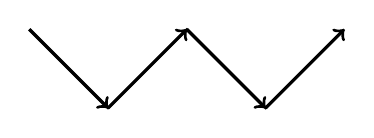
\begin{tikzpicture}
		% define point
		\coordinate (A)  at (1, 1);
		\coordinate (O)  at (2, 0);
		\coordinate (B)  at (3, 1);
		\coordinate (C)  at  (4,0);
		\coordinate (D) at  (5,1);
		% angle  
		\draw[thick] (A) -- (O) -- (B) -- (C)-- (D);
		%	\draw pic[draw=black,eccentricity=2.9]
		%\pic [draw,"$\alpha_1$",angle radius=20,->,angle eccentricity=1.4]
		%  {angle = B--O--A};
		\draw [->, very thick] (1,1) -- (2,0)  node [midway, above] {\scriptsize };
		\draw [->, very thick] (2,0) -- (3,1)  node [midway, above] {\scriptsize };
		\draw [->, very thick] (3,1) -- (4,0)  node [midway, above] {\scriptsize };
		\draw [->, very thick] (4,0) -- (5,1)  node [midway, above] {\scriptsize };
	\end{tikzpicture}
	\captionof{figure}{\textbf{Wing Gesture}}
	\label{Fig:5.9}
\end{center}

\begin{figure}[H]\centering
	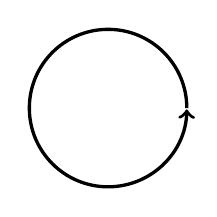
\begin{tikzpicture}
		\draw[->,very thick] (0,0) arc[radius=1cm,start angle=0,delta angle=359];
	\end{tikzpicture}
	\captionof{figure}{\textbf{Ring Gesture }}
	\label{Fig:5.10}
\end{figure}

\begin{figure}[H]\centering
	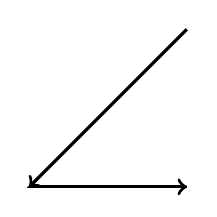
\begin{tikzpicture}
		% define point
		\coordinate (A)  at (2, 2);
		\coordinate (O)  at (0, 0);
		\coordinate (B)  at (2, 0);
		% angle  
		\draw[thick] (A) -- (O) -- (B);
		%\draw pic[draw=black,angle radius=20,angle eccentricity=1.4]
		%{angle = B--O--A};
		%\pic [draw,"$\alpha_1$",angle radius=20,->,angle eccentricity=1.4]
		%  {angle = B--O--A};
		\draw [->, very thick] (2,2) -- (0,0)  node [midway, above] {\scriptsize };
		\draw [->, very thick] (0,0) -- (2,0)  node [midway, above] {\scriptsize };
	\end{tikzpicture}
	\captionof{figure}{\textbf{Slope Gesture }}
	\label{Fig:5.11}
\end{figure}

\subsection{Regression}

In a regression task, the CNN output is a continuous numerical value. The network is designed to predict a specific numerical outcome, and the final layer often uses an activation function, such as linear, that allows for unbounded output. The training process involves minimizing the difference between the predicted value and the actual target value, as determined by the chosen loss function \cite{Xu:2022}.


\subsection{Output of the Model for Magic Wand}
\label{subsection:outputCNN}

The CNN functions as a classifier, producing class probabilities as its output. The final outcome is determined by the softmax layer \ref{Softmax Function}, resulting in a set of numerical values corresponding to different gesture categories. For example, if the magic wand project involves recognizing gestures like "swirl," "tap," "circle," and "wave," the model might output probabilities such as \texttt{[0.05, 0.70, 0.10, 0.15]}.

Each number in the output array represents the model's confidence score for a specific gesture category, and the category with the highest score is considered the model's prediction for the given input gesture. In the provided example, the model predicts that the gesture category "tap" is the most likely result with a confidence score of 0.70.

To enhance the reliability of gesture recognition, postprocessing techniques can be applied. Methods like score averaging or consensus-based recognition are commonly used. Averaging scores over multiple runs contributes to a more stable and consistent output, improving the model's ability to adapt to variations in gesture patterns and environmental conditions \cite{War:2020}.

Upon successful recognition of a gesture, the magic wand's command responder can utilize the device's output capabilities, triggering actions such as changing LED colors, producing sounds, or initiating specific functions. The two-dimensional structure of the model's output, aligning with the first dimension as a wrapper and the second holding probabilities for each gesture class, is designed to suit the requirements of the embedded hardware implementation on Arduino Nano 33 BLE Sense \cite{Set:2023}.

\subsubsection{The Softmax Function}
\label{Softmax Function}
The softmax function is commonly used in Convolutional Neural Networks (CNNs) and other machine learning models, particularly in the output layer, to convert a vector of raw scores or logits into probabilities. It essentially normalizes the input values into a probability distribution that sums to 1 \cite{Sewak:2018}.

In the context of CNNs, the softmax function is often applied to the output layer when the network is used for classification tasks. Here's the formula for the softmax function \cite{Win:2023}:

\begin{equation}
	\text{Softmax}(x_i) = \frac{e^{x_i}}{\sum_{j=1}^{K} e^{x_j}}
\end{equation}

Wwhere $x_i$ is the raw score or logit for class $i$, $K$ is the total number of classes, and $e$ is the base of the natural logarithm (Euler's number). An exmple of applying the Softmax function is shown in the Figure \ref{fig:softmax}.

\begin{figure}[h!]
	\centering
	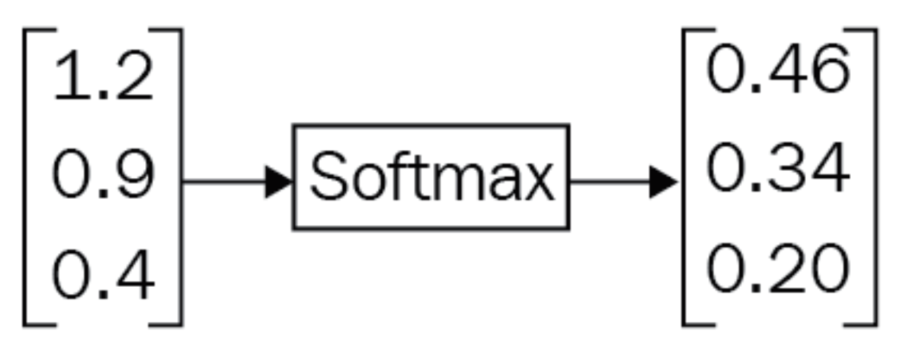
\includegraphics[width=0.4\textwidth]{Images/DataMining/softmax}
	\caption{Example of applying the softmax function \cite{Sewak:2018}} \label{fig:softmax}
\end{figure}


\section{Python Example Code}
\label{section:DataMiningExampleCode}


The identification of regional patterns within an image is facilitated by the convolutional layer. Following the convolutional layer, the max pooling layer is employed to diminish dimensionality. This section illustrates image classification by using a code provided by Sewak et al \cite{Sewak:2018}.

It is crucial to initially standardize all images to a uniform size. The initial convolution layer necessitates an additional parameter, \PYTHON{input.shape()}. The focus here is on training a Convolutional Neural Network (CNN) for image classification using the CIFAR-10 database. CIFAR-10 comprises 60,000 color images, each of size $32 \times 32$. These images are categorized into 10 classes, with 6,000 images per category, namely airplane, automobile, bird, cat, dog, deer, frog, horse, ship, and truck.

\subsection{Imports}

In the Listing \ref{code:cnnImports} are the necessary libraries and modules required for working with neural networks, image data, and visualization. The versions are shown in the Table \ref{tab:cnnlibraryVersions}.

\begin{itemize}
	\item Python version: 3.9.
\end{itemize}

\begin{table}[htbp]
	\centering
	\caption{Versions of Libraries}
	\label{tab:cnnlibraryVersions}
	\begin{tabular}{|l|c|}
		\hline
		\textbf{Library} & \textbf{Version} \\
		\hline
		Numpy & 1.23.5 \\
		Matplotlib & 3.7.1 \\
		Keras & 2.12.0 \\
		\hline
	\end{tabular}
\end{table}

\begin{code}[h!]
	\lstinputlisting[language=Python, numbers=none, linerange={82-89}]{Code/CNN/CNNDataMining.py}    
	
	\caption{Importing necessary libraries and modules.}
	\label{code:cnnImports}
\end{code}

\subsection{Load CIFAR-10 Dataset}

In Listing \ref{code:cnnLoadCifar} the CIFAR-10 dataset is loaded.CIFAR-10 is a dataset of 50,000 $32 \times 32$ color training images and 10,000 test images.

\begin{code}[h!]
	\lstinputlisting[language=Python, numbers=none, linerange={107-107}]{Code/CNN/CNNDataMining.py}    
	
	\caption{Loading and preparing the CIFAR-10 dataset.}
	\label{code:cnnLoadCifar}
\end{code}

\subsubsection{Data Preprocessing}

In the Listing \ref{code:cnnDataPreprocessing} the image data is normalized and one-hot encoding is performed on the labels. The training set is split into training and validation sets.

\begin{code}[h!]
	\lstinputlisting[language=Python, numbers=none, linerange={124-133}]{Code/CNN/CNNDataMining.py}    
	
	\caption{Preprocessing data: normalization, one-hot encoding, and splitting into training and validation sets}
	\label{code:cnnDataPreprocessing}
\end{code}

\subsection{Augmented Image Generator}

In the Listing \ref{code:cnnAugmentedGenerator} image data generators for training and validation is created and configured. These generators will perform data augmentation, such as shifting and flipping, to increase the diversity of the training set.

\begin{code}[h!]
	\lstinputlisting[language=Python, numbers=none, linerange={154-168}]{Code/CNN/CNNDataMining.py}    
	
	\caption{Configuring image data generators for augmentation and fitting them on training and validation data}
	\label{code:cnnAugmentedGenerator}
\end{code}

\subsection{Plot the First Nine Images of Cifar-10}

Listing \ref{code:cnnPlotCifar10} loads the cifar-10 dataset and plots the first nine images as shown in Figure \ref{fig:cnnFirstNineCifar10}.

\begin{code}[h!]
	\lstinputlisting[language=Python, numbers=none, linerange={177-183}]{Code/CNN/CNNDataMining.py}    
	
	\caption{Loading and visualizing the first nine images from the CIFAR-10 dataset}
	\label{code:cnnPlotCifar10}
\end{code}

\begin{figure}[h!]
	\centering
	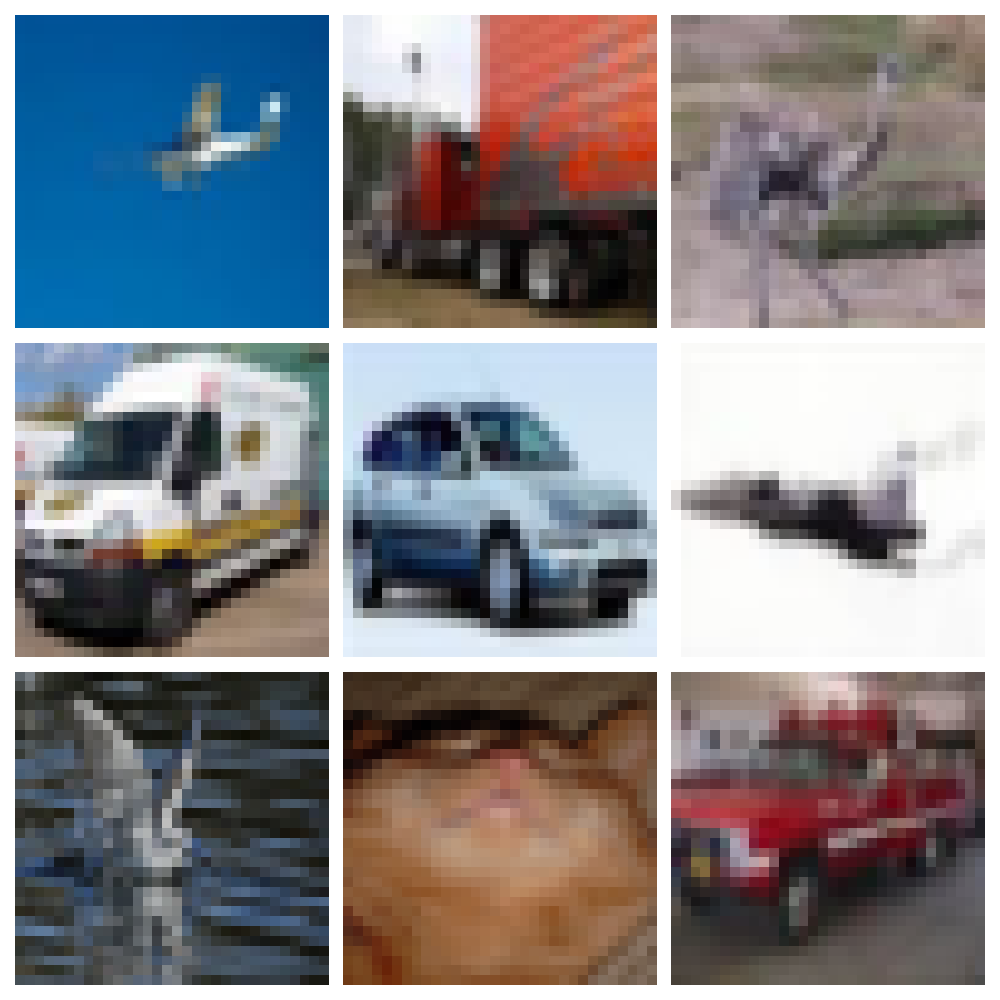
\includegraphics[width=0.8\textwidth]{Images/DataMining/CIFAR10SecondNineImages}
	\caption{First nine images from the CIFAR-10 dataset.} \label{fig:cnnFirstNineCifar10}
\end{figure}

\subsection{CNN Model Definition}

A Convolutional Neural Network (CNN) model is defined in Listing \ref{code:cnnDefinition} using Keras with convolutional layers, max pooling, dropout for regularization, and dense layers.

\begin{code}[h!]
	\lstinputlisting[language=Python, numbers=none, linerange={199-207}]{Code/CNN/CNNDataMining.py}    
	
	\caption{Defining a Convolutional Neural Network (CNN) model using Keras}
	\label{code:cnnDefinition}
\end{code}

\subsection{Compile the Model}

In Listing \ref{code:cnnCompileModel} the model is compiled with the specified loss function, optimizer, and evaluation metric.

\begin{code}[h!]
	\lstinputlisting[language=Python, numbers=none, linerange={223-223}]{Code/CNN/CNNDataMining.py}    
	
	\caption{Compiling the CNN model with specified loss function, optimizer, and metric}
	\label{code:cnnCompileModel}
\end{code}

\subsection{Train the Model with Augmented Data}

In Listing \ref{code:cnnTrainAugmented} the model is trained using the augmented data generators. This involves calling the \PYTHON{fit\_generator} function instead of \PYTHON{fit} and providing the data generators for training and validation sets.

\begin{code}[h!]
	\lstinputlisting[language=Python, numbers=none, linerange={238-247}]{Code/CNN/CNNDataMining.py}    
	
	\caption{Training the CNN model with augmented data using data generators}
	\label{code:cnnTrainAugmented}
\end{code}

\subsection{Plotting the Loss and Accuracy Curves}

In Listing \ref{code:cnnLossAccuracyPlot} the accuracy and loss curves are plotted. The results are shown in the Figure \ref{fig:AccuracyandLoss}. The observed trends in the training and validation metrics, with a downward trend in both training and validation loss and an upward trend in accuracy, indicate positive learning and generalization behavior of the neural network. The somewhat unconventional scenario of validation loss being below training loss and validation accuracy exceeding training accuracy could be influenced by effective data augmentation, contributing to the model's robustness. These trends collectively suggest that the model is not overfitting the training data and is likely to generalize well to unseen data, highlighting successful training and potential for further improvement.

\begin{code}[h!]
	\lstinputlisting[language=Python, numbers=none, linerange={263-284}]{Code/CNN/CNNDataMining.py}    
	
	\caption{Plotting the loss and accuracy curves}
	\label{code:cnnLossAccuracyPlot}
\end{code}

\begin{figure}[h!]
	\centering
	
	\begin{subfigure}{0.45\textwidth}
		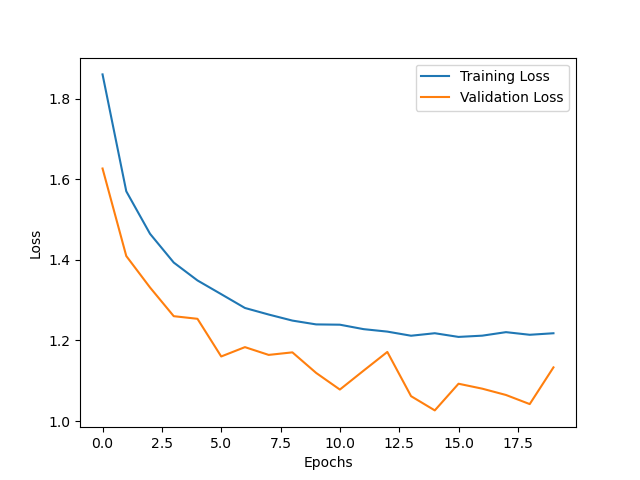
\includegraphics[width=\linewidth]{Images/DataMining/lossPlot}
		\caption{}    % \caption{} is kept to keep (a), (b), (c) etc. below each subfigure.
		\label{subfig:lossTrends}
	\end{subfigure}
	\hfill
	\begin{subfigure}{0.45\textwidth}
		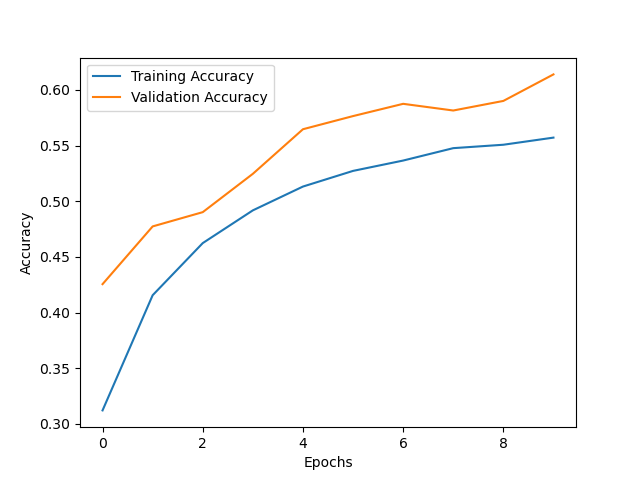
\includegraphics[width=\linewidth]{Images/DataMining/accuracyPlot}
		\caption{}    % \caption{} is kept to keep (a), (b), (c) etc. below each subfigure.
		\label{subfig:accuracyTrends}
	\end{subfigure}
	
	\caption{(\subref{subfig:DigitalImage}) Training and validation loss trends over epochs. (\subref{subfig:DigitalImagePixelValues}) Training and validation accuracy trends over epochs.}
	\label{fig:AccuracyandLoss}
\end{figure}

